\newcommand{\Title}{WAK-Lab FAQ} 
\title{\Title}

\documentclass[a4paper]{article}
\usepackage{geometry}
\geometry{a4paper,tmargin=25mm,bmargin=35mm,lmargin=20mm,rmargin=20mm,footskip=5mm}
\usepackage[utf8]{inputenc}
%\usepackage[T1]{fontenc}
\usepackage{fontspec}
\usepackage{graphicx}
\usepackage{subcaption}
%\usepackage{picins}
\usepackage{capt-of}
\usepackage{lastpage}
\usepackage[ngerman]{babel}
\usepackage[colorlinks=true,linkcolor=black,urlcolor=black]{hyperref}
%\usepackage[headtopline,headsepline,footsepline,footbotline]{scrpage2}
%\usepackage[headtopline,headsepline]{scrpage2}
\usepackage[headsepline,footsepline]{scrpage2}
\usepackage{multirow}
\usepackage{listings}            
% fuer Stichwortverzeichnis
\usepackage{makeidx}
%\usepackage[automark,headsepline,footsepline,plainheadsepline,plainfootsepline]{scrpage2}

\usepackage{xcolor,soul}
\usepackage{colortbl} % Farbige Tabellen

\usepackage{longtable}

\usepackage{tabularx}
%\setheadtopline{.5pt}
%\setheadsepline{.5pt}

\pagestyle{scrheadings}
\clearscrheadfoot

%%standard commands
\newcommand{\ltab}{\raggedright\arraybackslash} % Tabellenabschnitt linksbündig
\newcommand{\ctab}{\centering\arraybackslash} % Tabellenabschnitt zentriert
\newcommand{\rtab}{\raggedleft\arraybackslash} % Tabellenabschnitt rechtsbündig


%%Kopfzeile
\ihead{{\textbf{\large \Title}}}
%\chead{\textbf{\large \title}}
\ohead{\raisebox{0.1\totalheight}{
\includegraphics[width=0.15\textwidth]{pictures/wak-lab-LOGO.png}}}

%%Fu\ss zeile
\cfoot{\pagemark}
\ofoot{\today}

   

\begin{document}
\maketitle
%\tableofcontents
\begin{center}

\includegraphics[height=10cm]{pictures/wak-lab-profilbild.jpg}
\end{center}
\vspace{2cm}
\fbox{\parbox[c][6cm][c]{\textwidth}{
%\section*{Shortcuts}
\begin{itemize}
  \item Website: \url{https://www.wak-lab.org}
  \item Paypal Moneypool: \url{https://paypal.wak-lab.org}
  \item Discord Server: \url{https://dc.wak-lab.org}
  \item Gitlab Server: \url{https://git.wak-lab.org}
  \item Nextcloud: \url{https://nc.wak-lab.org}
  \item FAQ: \url{https://github.com/thehilde/Wak-Lab-Docs/blob/master/FAQ/FAQ.pdf?raw=true}
  \item WA: \url{https://chat.whatsapp.com/EGc0lJaG8x9JUUz9530W5N} 
\end{itemize}
}}
\newpage
%\tableofcontents
%\newpage
%\section*{Vorwort}
\section{Einführung}
Viele haben lange darauf gewartet, in Eisenach hat sich erstmals am 11. Januar  2019 eine Gruppe von 12 technisch interessierten Menschen getroffen. Sie wollen sich auch zukünftig regelmä\ss ig treffen. Es soll gemeinsam gebastelt, gelötet und programmiert werden.\\
\ \\
Zunächst haben wir uns drauf verständigt diese Treffen regelmäßig in der alten Posthalterei (Abb. \ref{img:ESAPOSTHALTEREI}) abzuhalten. Dabei werden uns die Räumlichkeiten stundenweise überlassen.\\
\ \\
\begin{minipage}[t]{\textwidth}
  \centering
  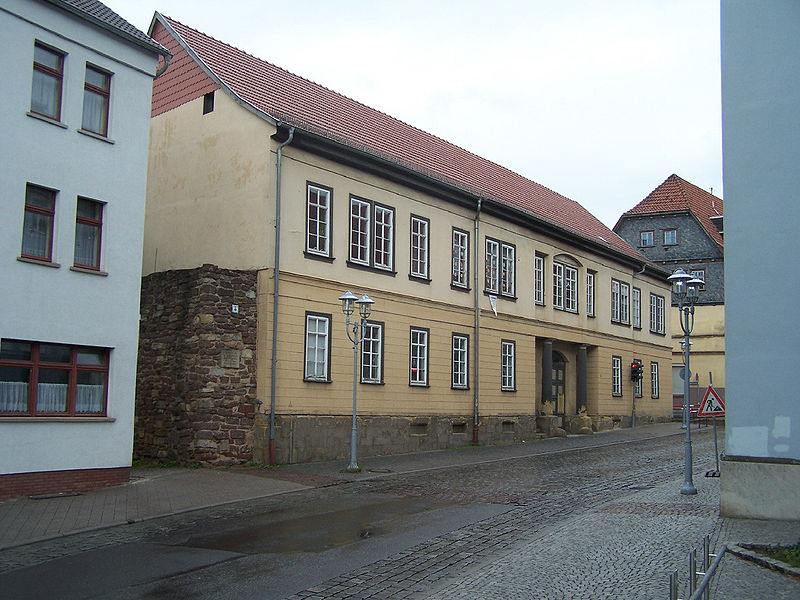
\includegraphics[height=6cm]{pictures/800px-ESAPOSTHALTEREI.jpg}
  \captionof{figure}{Alte Posthalterei}
  \label{img:ESAPOSTHALTEREI}
\end{minipage}
\ \\
Wir wollen mit einer Präsenz in sozialen Medien und mit einem Flyer (Abb. \ref{img:FlyerMitPlatine}) zunächst andere Menschen auf unsere Idee aufmerksam machen. Das weitere Vorgehen ist von der Resonanz abhängig. Ideen über Vereinsgründung und Gemeinnützigkeit bestehen, aber wir wollen bewusst dieses Thema zunächst vertagen. \\
\ \\
\begin{minipage}[t]{0.5\textwidth}
  \centering
  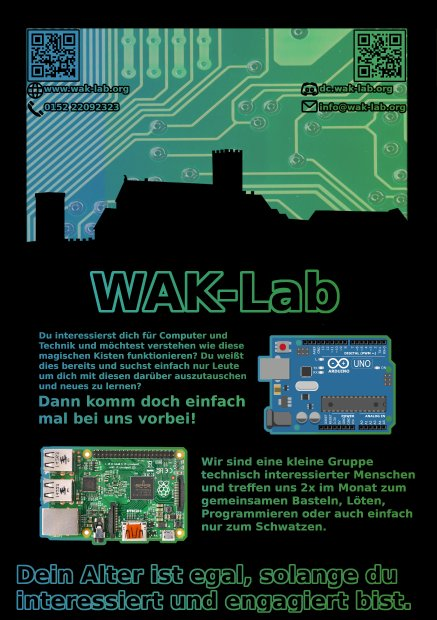
\includegraphics[height=6cm]{pictures/FlyerMitPlatine.jpg}
  \captionof{figure}{Flyer}
  \label{img:FlyerMitPlatine}
\end{minipage}
\begin{minipage}[t]{0.5\textwidth}
  \centering
  
\includegraphics[height=6cm]{pictures/FlyerRueckseite.jpg}
  \captionof{figure}{Flyer Rückseite}
  \label{img:FlyerRueckseite}
\end{minipage}

\subsection{Finanzierung}
Solange wir noch eine lose Interessensgemeinschaft sind sammeln wir bei PAYPAL \url{https://paypal.me/pools/c/8bkJSaWWlD} Geld für Flyer und andere notwendigen Ausgaben. Die Beteiligung ist freiwillig. Das Geld wird transparent und demokratisch ausgegeben. Eine übersicht über die Finanzen findet ihr unter Nextcloud\textbackslash Wak-Lab\textbackslash Finanzen 2019.ods. Sachspenden die für den Betrieb der Infrastruktur benötigt werden, sind ebenso willkommen. \\
\ \\
\textbf{Hinweis:} Es versteht sich, dass Geld- und Sachspenden nach Vereinsgründung in dessen Eigentum übergeht.\\

\subsection{Abstimmungen}
Abstimmungen werden zunächst über \url{http://www.strawpoll.me} durchgeführt.\\

\begin{minipage}[t]{\textwidth}
  \centering
  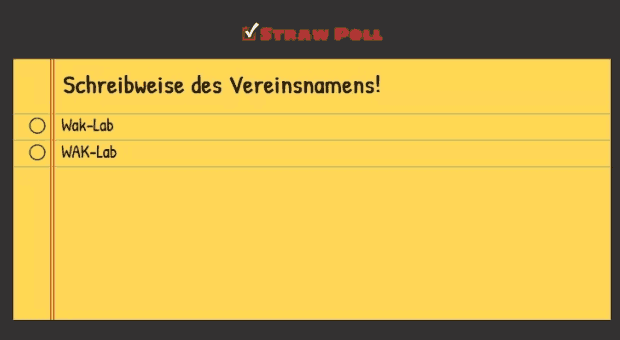
\includegraphics[height=6cm]{pictures/StrawPoll.png}
  \captionof{figure}{Online Abstimmung}
  \label{img:StrawPoll}
\end{minipage}


\newpage

 

\section{E-mail}
E-Mails an das WAK-Lab richtet ihr bitte an \url{info@wak-lab.org}. Wer Zugriff auf das Postfach benötigt, einen eigenen Account oder einen Zugang zur Nexcloud kann sich hierhin wenden.\\

\section{Nextcloud}
Über die URL \url{https://nc.electribez.de/index.php/login} kommt ihr zur Verwaltungskonsole auf unserem Raspi-Nextcloud Server. Dort könnt ihr euer Password ändern, welches ihr vom Admin zugewiesen bekommen habt.\\

\begin{minipage}[t]{\textwidth}
  \centering
  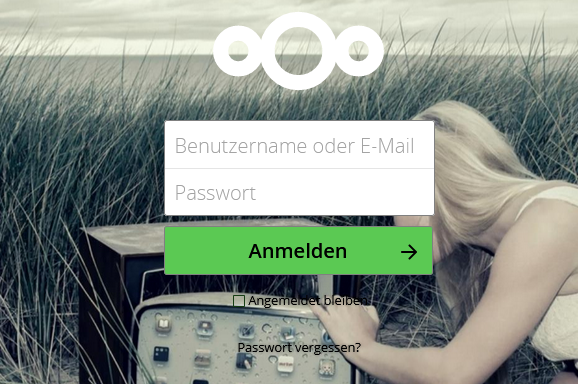
\includegraphics[height=5cm]{pictures/Nextcloudlogin.png}
  \captionof{figure}{Nextcloud Login}
  \label{img:Nextcloudlogin}
\end{minipage}


\subsection{Client Installieren}
Passende Clienten findet ihr auf \url{https://nextcloud.com/install/}\\
\ \\
Der Nexcloud Clienent stellt euch einen ständig Aktualisierte Kopie des Servers in C:\textbackslash Users\textbackslash Username\textbackslash Nextcloud zur Verfügung. Dort können wir gemeinsam an Inhalten arbeiten. Vorsicht, wenn 2 Leute an einen Thema arbeiten.\\
 
\begin{minipage}[t]{\textwidth}
  \centering
  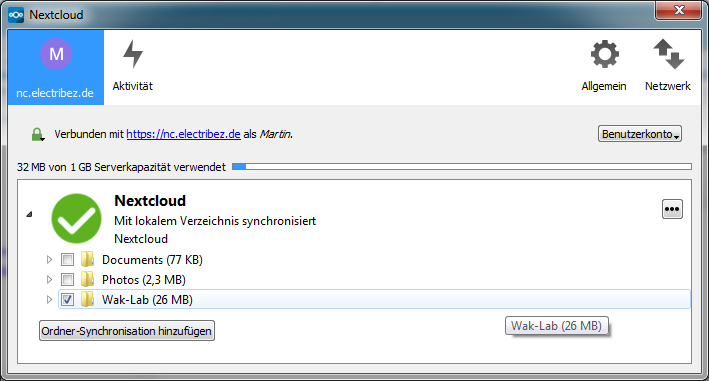
\includegraphics[height=5cm]{pictures/NextcloudWinClient.png}
  \captionof{figure}{Nextcloud Windows Client}
  \label{img:NextcloudWinClient}
\end{minipage}






\section{Discord}
Wenn ihr mit Discord arbeiten wollt, benötigt ihr eine Discord Client App mit der erstellt ihr einen Discord Account. Dabei wird wird Nickname, Email und Passwort benötigt. Ihr könnt dann sofort Loslegen und den Link zu unserem Discod Server Klicken und eich mit underem Server verbinden. URL: \url{https://dc.wak-lab.org} Alternativ: \url{https://discord.gg/FUJuq4h}\\
\ \\
Nach der Registrierung kommt eine Bestätigungs E-Mail in euer Postfach, das könnt ihr dann ja noch abschließen. Evtl. landet die Mail im Spam Ordner. \\

\ \\
\begin{raggedright}
\begin{tabular}{|p{7,3cm}|p{7,3cm}|}
\hline
\textbf{Channel} & \textbf{Beschreibung}\\
\hline
\#wak-lab\_talk & Gruppenchat\\
\hline
\#wak-lab\_verein & Geschlossene Gruppe\\
\hline
\#wak-lab\_vorstand & Geschlossene Gruppe\\
\hline
\#events & Gruppenchat\\
\hline
\#ankündigungen & Nächste Schritte\\
\hline
LAB TOPIC & Allgemeine Themen\\
\cline{1-1}
\#windows & \\
\cline{1-1}
\#linux & \\
\cline{1-1}
\#develop & \\
\cline{1-1}
\#funk\_radio\_sdr & \\
\cline{1-1}
\#3d-druck & \\
\cline{1-1}
\#smart-home & \\
\cline{1-1}
\#werkstatt & \\
\hline
ELEKTRONIK & Elektronik Themen\\
\cline{1-1}
\#electronik & \\
\cline{1-1}
\#arduino & \\
\cline{1-1}
\#esp8266\_und\_co & \\
\cline{1-1}
\#raspberry-pi & \\
\hline
\end{tabular}
\captionof{table}{Liste der Channels}
\label{tab:Channels}
\end{raggedright}



\section{Git und SVN}
Vorweg will ich kurz erklären, was es mit den Tools zur Versionskontrolle auf sich hat.\\
\ \\
Es geht immer darum, eine lokale Kopie der Quellen von einem Server zu laden. Im einfachsten Fall bei Github als ZIP-Datei. Dies ist in den meisten Fälle ausreichend. Der Link ist jedoch für unsere Versionskontrolle interessant. Dort liegt nun das Repository die ich nenne sie jetzt mal Masterkopie. \\
\begin{minipage}[t]{\textwidth}
  \centering
  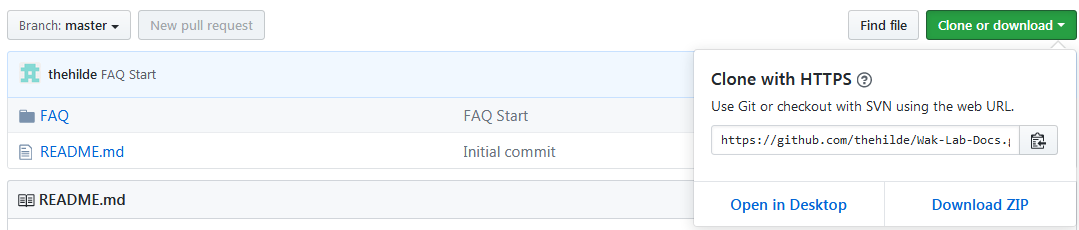
\includegraphics[width=\textwidth]{pictures/Clone.png}
  \captionof{figure}{Eine lokale Kopie Clonen}
  \label{img:Clone}
\end{minipage}
\ \\
Spannend wird es jedoch, wenn die Quellen sich auf dem Server weiterentwickeln oder man sogar selbst eine Verbesserung einbringen will. Die Tools GIT oder SVN managen nun die Synchronisation mit dem Server. Es kann der zeitliche Verlauf der Änderungen angezeigt und zu beliebigen Punkten zurück gesprungen werden. Nie wieder ein "Gestern ging es noch bevor das umgestrickt habe <aarg!>". Welche Änderungen habe ich vor 3 Jahren für XY rein gehackt? Und vor allem Warum? Welchen Fehler wollte ich beseitigen, welches Ticket habe ich bearbeitet? Oder war es der Kollege?  \\
Tools wie Tortoise SVN besitzen eine Explorer Integration, arbeiten über das Kontextmenü und zeigen alle Änderungen automatisch an. \\
\begin{minipage}[t]{\textwidth}
  \centering
  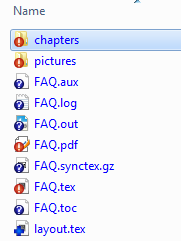
\includegraphics[height=3cm]{pictures/TortoiseSVNChanges.png}
  \captionof{figure}{Tortoise SVN Explorer Integration}
  \label{img:TortoiseSVNChanges}
\end{minipage}
\ \\
Finden Änderungen in der selben Datei aber in unterschiedlichen Bereichen statt, kann das Tool die Änderungen automatisch zusammenführen. In manchen Fällen muss dies jedoch händisch erfolgen.\\
\ \\
Es soll noch gesagt sein, das GIT und SVN zwei verschiedene Tools sind, die etwas abweichende Philosophien haben. Zum Glück sind die beiden auf Github gut verheiratet worden.\\
\ \\
Folgende Dateitypen sind Textbasiert und können prima verwaltet werden.
\begin{itemize}
\item Arduino .ino Dateien
\item Quelltexte z.B. .c .cpp .h .pas .vhdl
\item Natürlich .html .php
\item Windows .ini Dateien
\item Eagle Layout Dateien und Bibliotheken ab Version 6
\item STM Cube32 Dateien
\item \LaTeX .tex Dateien
\item Auch Word ist Prima integriert in Tortoise SVN und öffnet den Word eigenen DIF Viewer.
\end{itemize}


  






\section{\LaTeX}
Latex ermöglicht es aus Textdateien formatierte PDF Dokumente zu erstellen. Ähnlich der Buchfunktion im Wikipedia. Außerdem können Ausgaben von Programmen ansprechend formatiert ausgegeben werden.\\
Durch das Einbinden von externen Dateien können Textbausteine, Layouts oder Bilder zentral abgelegt werden. Beispielsweise können dadurch Layout, Adresse oder Logo eines Vereins einfach in allen Dokumenten gleichzeitig verändert werden. Die Dokumente müssen nur neu compiliert werden.\\
Ich verwende als Editor den Texmaker und als Latex Distribution Miktex. Sollte es dazu Fragen geben einfach mal an mich wenden.\\

\begin{minipage}[t]{\textwidth}
  \centering
  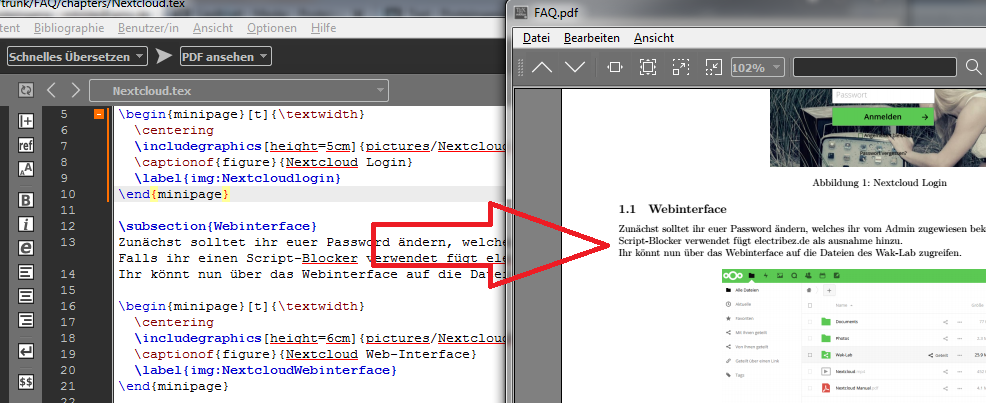
\includegraphics[width=\textwidth]{pictures/Texmaker.png}
  \captionof{figure}{Texmaker}
  \label{img:Texmaker}
\end{minipage}




\end{document}


